% =====================================================================
% ARR October 2026 cycle  (submission deadline Oct 12 2026)
% Style files are the UNMODIFIED official ACL copies from
%   github.com/acl-org/acl-style-files (master).
%   acl.sty  md5 e2c027f483aa40e577ed34264c8b0655
% DO NOT edit acl.sty, and do not use \setlength\titlebox below 5cm,
% \raggedbottom, \enlargethispage or any other spacing hack. A previous
% submission of this work was desk rejected for exactly that.
%
% VERIFIED ARR/ACL RULES (aclrollingreview.org/authors + ACLPUB formatting):
%   long paper REVIEW version : 8 pages of CONTENT (9 on acceptance)
%   references                : UNLIMITED, do not count
%   appendices                : do not count, no maximum total PDF length
%   "Limitations" section     : REQUIRED, does NOT count toward the limit
%   Ethics / Broader Impact   : optional, does NOT count
% So the budget to manage is 8 pages up to the start of Limitations.
% =====================================================================
\documentclass[11pt]{article}
\usepackage[review]{acl}

\usepackage{times}
\usepackage{latexsym}
\usepackage[T1]{fontenc}
\usepackage[utf8]{inputenc}
\usepackage{microtype}
\usepackage{inconsolata}
\usepackage{graphicx}
\usepackage{booktabs}
\usepackage{amsmath}
\usepackage{amssymb}
\graphicspath{{figures/}}

\title{When Debiasing Scores Reward Broken Text}

\author{Anonymous ARR submission}

\begin{document}
\maketitle

\begin{abstract}
Activation steering for social bias is judged by a target metric that rewards the absence
of the vocabulary marking the bias. We show that broken text satisfies this metric, and
that the methods with the strongest reported scores are the ones it flatters most. An
exploratory sweep of five steering methods on a disability-bias benchmark (21{,}750
generations) finds three that reach the metric's value for
unbiased text while emitting corrupted or repeated responses, through failure modes that
no single filter on emptiness, length or uniqueness detects. A pre-registered test on 50
held-out questions, scored by judges from two model families, confirms this. The method with
the largest effect size pushes the model past neutral and loses two points of judged
quality out of ten, and SADI's published setting leaves a fifth of its responses
unparseable, under both judges. A system prompt instructing the model not to medicalize
removes only $13\%$ of the bias, so steering is still needed, and the two combine: the
prompt together with a multi-rank projection removes $97\%$ of medicalization with no
degenerate output, more than any single method achieves intact. Finally, the spectral
statistic used to describe a bias's dimensionality reports how the contrast set was built: holding 13 pairs fixed and varying only prompt diversity moves the top
explained-variance ratio from $22\%$ to $76\%$.
\end{abstract}

% =====================================================================
% BRANCH B DRAFT: Sections 1 and 4
% Working title: When Debiasing Scores Reward Broken Text
% Target: ARR October 2026 cycle (submission Oct 12) -> NAACL/COLING 2027
%
% STATUS: first draft for author review. Citations marked
% [CITATION NEEDED] were NOT programmatically verified and must be
% checked before submission. Verified-real citations are noted inline.
% =====================================================================

\section{Introduction}

Ask a language model how to start a fitness routine and it answers the
question. Mention a disability in the same query and it often answers a
different one: consult your physician, be mindful of your limitations,
consider the risks. The user asked about exercise and was handled as a
patient. This pattern, which we call medicalization bias following
\citep{accesseval2024}, appears across domains that have nothing to do with
medicine, including credit cards, air travel, and film distribution.

Activation steering offers a way to remove such behaviour at inference time,
by editing the model's internal activations with no retraining
\citep{turner2023activation,rimsky2024steering}. Whether an intervention
works is judged by a target metric: how much less often the steered model
produces the vocabulary that marks the bias. We set out to reduce
medicalization bias this way, and the results we report here are what we
found about how that judgment is made.

On the AccessEval disability-bias benchmark \citep{accesseval2024}, the
strongest target-metric score in our comparison belongs to SADI
\citep{wang2025sadi}. At its reported operating point it scores zero, the
metric's value for unbiased text, on 201 of 250 responses. Those responses
are not absent. They average 188 words and read like this: ``Improving
digital security for individuals with mental\texttt{GuidId\&ampHeaderCode}
Behavioral\texttt{HeaderCode} Disorders\ldots'' The medicalization metric is
a log-odds contrast between medical and professional vocabulary, and
corrupted text contains neither, so the contrast evaluates to zero and the
metric records perfect neutrality.

FairSteer \citep{li2025fairsteer} fails the same way at higher strength but
with a different signature: at $\alpha{=}6$ only 68 of its 250 responses are
distinct, and the most frequent one, returned verbatim for 43 different
prompts, is the word ``Here'' repeated for 1{,}048 words. It too scores zero.
Angular Steering \citep{vu2025angular} reaches the highest effect size in our
comparison while injecting corruption inside words, and pushes past neutral,
which withholds medical information from users who asked for it.

These methods sit at the top of a leaderboard. None of them has reduced
medicalization bias.

This is the problem we address. The metric counts an absence, and an
intervention can produce that absence either by removing the bias or by
destroying the answer. Nothing in the standard evaluation separates the two,
and the degenerate outputs are not obviously degenerate: they are fluent in
shape, correctly formatted, and longer than the baseline responses they
replace. A practitioner comparing published numbers would select one of these
methods, deploy it, and ship a model that answers disability-related queries
with corrupted or repeated text. The users who carry that cost are the ones
the intervention was meant to protect.

The same weakness appears a second time, one step earlier in the pipeline.
Recent methods set the \emph{structure} of an intervention, in particular its
rank, from the singular value spectrum of contrastive activation differences
\citep{zou2023representation}. % HiDRA, SAE-SSV, CAS-BiPO: [CITATION NEEDED], all three verified real, BibTeX not yet fetched
A concentrated spectrum is read as a behaviour that one direction can
address, a diffuse one as a behaviour that needs many. We show that this
statistic reports how the contrastive set was built rather than how the
behaviour is represented. Holding the number of pairs fixed at 13 and
varying only the diversity of the prompts moves the top explained-variance
ratio from $22.1\%$ to $76.1\%$, on one benchmark, at one layer.

Both failures have the same shape. A quantity is treated as a measurement of
the bias, and it is measuring something else: output length in the first
case, prompt diversity in the second. We establish this for both quantities
and show what changes once it is corrected. Under a quality-constrained
comparison the ranking of steering methods changes, and a multi-rank
projection reduces medicalization as far as the strongest rank-1 baseline
while keeping the answers intact.

Our contributions:

\begin{itemize}
\item \textbf{An evaluation audit of six steering methods.} We show that
  two of the three highest target-metric scores come from collapsed or
  corrupted generations, and we give the failure modes at token level
  (Section~\ref{sec:audit}).
\item \textbf{A quality-constrained comparison on matched items.} On an
  identical $n{=}250$ AccessEval subset with a shared baseline, the
  multi-rank projection reaches $d{=}0.337$ against CAA's $d{=}0.341$
  while degrading judged quality significantly less (paired difference
  $+0.35$ on a ten-point scale, $95\%$ CI $[0.18, 0.53]$, Wilcoxon
  $p<0.001$).
\item \textbf{Rank matters for the intervention.} Holding the layer, the
  data, and the operator fixed, rank-1 erasure fails ($d{=}{-}0.03$) where
  a rank-40 erasure recovers $d{=}0.205$ (Section~\ref{sec:rank}).
\item \textbf{Measured bias dimensionality is a property of the contrast
  set.} Four controls (prompt homogeneity, cluster versus pair sampling,
  a permutation null, and a cluster bootstrap) show that the spectral
  statistics used to describe ``bias geometry'' track contrast-set
  construction rather than bias type (Section~\ref{sec:geometry}).
\end{itemize}



% =====================================================================

% Section 2: the evaluation audit. Every number verified against the saved sweep results
% (~/Downloads/{sadi_results-2,fairsteer_results_L29,caa_results_L14}.json).
\section{How a debiasing score is earned}
\label{sec:audit}

The medicalization score is a log-odds contrast between two halves of a vocabulary, the
medical and the professional \citep{monroe2008fightin}. A response drops toward zero when
it stops using medical words relative to professional ones. It also drops toward zero
when it stops using either, which is a different event with the same measurement.

This section is about how often the second event is what happened.

\paragraph{Three ways to score zero.} Table~\ref{tab:degeneration} gives the three
methods that reach a mean medicalization of $0.000$ on AccessEval, the metric's value for
unbiased text, along with what the responses look like at that point. The unsteered model
averages 481 words and scores $0.712$.

\begin{table}[t]
\centering\small
\begin{tabular}{lrrr}
\toprule
& SADI & FairSteer & CAA \\
& $s{=}10$ & $\alpha{=}6$ & $\alpha{=}6$ \\
\midrule
Medicalization & $0.119$ & $0.000$ & $0.000$ \\
Judged quality & $3.19$ & $2.38$ & $3.02$ \\
\midrule
Empty responses & $0$ & $0$ & $0$ \\
Mean length (words) & $188$ & $945$ & $638$ \\
Distinct of 250 & $249$ & $\mathbf{68}$ & $247$ \\
\bottomrule
\end{tabular}
\caption{Three methods at settings where the target metric reports success, and what the
responses are. No filter on emptiness, length or uniqueness catches all three: none
produces an empty response, all three are at or above the unsteered length of 481 words
except SADI, which is shorter but almost entirely distinct, and only FairSteer collapses
into repetition.}
\label{tab:degeneration}
\end{table}

The three failures are not variants of one another. SADI corrupts tokens inside words
while keeping the responses distinct, 249 of 250, so a uniqueness check passes it. A
typical response reads ``Improving digital security for individuals with
mental\texttt{GuidId\&ampHeaderCode} Behavioral\texttt{HeaderCode}
Disorders\ldots{}requires empathy, understanding,\texttt{HeaderCode} Viable IT
solutions, Viable IT Viable IT''. Of its 250 responses, 201 score exactly $0.000$.

FairSteer fails in the opposite direction. Only 68 of its 250 responses are distinct, and
the most frequent one, returned verbatim for 43 different prompts, is the word ``Here''
repeated for 1{,}048 words. CAA at the same nominal strength produces a third pattern,
247 distinct responses of 638 words each, built from looping phrases rather than a single
repeated token.

\paragraph{No cheap filter separates them.} The obvious guards each fail on at least two
of the three. Checking for empty output catches none: every response is non-empty.
Filtering on length catches none: FairSteer and CAA are more than twice the unsteered
length, and SADI's 188 words is short but well inside the range of a legitimate answer.
Counting distinct responses catches FairSteer alone. A reviewer applying any single one
of these and finding it clean would conclude the outputs were fine.

\paragraph{What this costs the ranking.} These are not obscure corners of the
hyperparameter space. SADI's published operating point is one of them, and it posts the
lowest medicalization score among the five methods we compare while losing $60\%$ of the
model's judged quality. The metric cannot distinguish the two events, so a practitioner
selecting a method from published numbers would choose the one that damages responses
most, and the users who carry that cost are the ones the intervention was built to
protect.

Section~\ref{sec:frontier} measures the quality axis explicitly and re-runs the
comparison with both axes visible.

% PORTED from paper_aaai2027/main.tex Method section (Phases 1,2,4), with Phase 3
% reframed: the decomposition still supplies the subspace, but we no longer claim the
% spectrum diagnoses a bias type. Section~\ref{sec:geometry} is why.
\section{Measuring and removing medicalization}
\label{sec:method}

\paragraph{The bias vocabulary.} The signal we measure is the differential frequency of
words across demographic groups, identified by log-odds ratios with informative
Dirichlet priors \citep{monroe2008fightin}. For groups $i$ and $j$ the log-odds ratio
for word $w$ is
\begin{multline}
\delta(w) = \log\frac{y_i^w + \beta^w}{n_i - y_i^w + \beta_0 - \beta^w} \\
- \log\frac{y_j^w + \beta^w}{n_j - y_j^w + \beta_0 - \beta^w}
\label{eq:logodds}
\end{multline}
where $y_i^w$ counts $w$ in group $i$'s responses, $n_i$ is that group's token count,
and $\beta^w$ is a prior proportional to background frequency. Words with $|z|>3.0$ form
the bias vocabulary. The threshold is not load-bearing: the top-20 vocabulary is
unchanged at $|z|>2.0$, $2.5$ and $3.0$ across six DiscrimEval lexicons. A response's
medicalization score is the log-odds contrast between the medical and professional
halves of this vocabulary, so a response containing neither scores zero. That property
is what Section~\ref{sec:audit} exploits.

\paragraph{Locating the layers.} We use layer-level activation patching at the residual
stream \citep{wang2022interpretability,conmy2023automated}: for each layer and component
we cache activations from a biased prompt, inject them into a neutral prompt's forward
pass, and measure whether the output moves toward the biased behaviour. Layers producing
significant shifts are the ones we intervene at. We call these a bias circuit only in
this layer-localization sense and do not perform edge-level attribution. A
\textit{loudness filter} then keeps the contrastive pairs whose clean-corrupted L2
distance exceeds the median, $\|\mathbf{h}_{\text{clean}} -
\mathbf{h}_{\text{corrupted}}\|_2 \geq p_{50}$, discarding pairs where the model barely
separates the groups. On AccessEval this keeps 2{,}083 of 4{,}164 pairs (1{,}044
distinct; the dataset lists every question twice).

\paragraph{The subspace.} At a circuit layer we take differences $\Delta \mathbf{h}_i =
\mathbf{h}_i^{\text{corrupted}} - \mathbf{h}_i^{\text{clean}}$ at the last token, centre
them, stack them into $\mathbf{M} \in \mathbb{R}^{n \times d}$, and factorise
$\mathbf{M} = \mathbf{U}\boldsymbol{\Sigma}\mathbf{V}^\top$. We steer with the top-$k$
right singular vectors $\mathbf{V}_k$. As an object this decomposition is close to
Linear Artificial Tomography \citep{zou2023representation}; what differs is that we use
$k$ components rather than one. We set $k{=}40$, the rank reaching $80\%$ of the
spectrum's variance on AccessEval. Section~\ref{sec:rank} shows that this choice is
doing real work, and Section~\ref{sec:geometry} shows what the spectrum does not
license us to infer from it.

\paragraph{The intervention.} We project activations onto the orthogonal complement of
$\mathbf{V}_k$ at the circuit layers with strength $\alpha$:
\begin{equation}
\mathbf{h}' = \mathbf{h} - \alpha \, \mathbf{V}_k \mathbf{V}_k^\top (\mathbf{h} - \boldsymbol{\mu})
\label{eq:steer}
\end{equation}
At $\alpha{=}1$ this is pure orthogonal projection; $\alpha>1$ reflects and scales the
in-subspace component. We report $\alpha{=}1$ throughout and sweep $\alpha$ only to
locate the point at which the operator breaks (Section~\ref{sec:frontier}). Intervening
at a single layer leaks, reducing medicalization by $16.8\%$; applying
Eq.~\ref{eq:steer} at both circuit layers at once (L21 and L25 for AccessEval) reaches
$71.6\%$. During prefill we steer only the last token, and during generation every newly
produced token \citep{li2024inference,todd2024function}.

% =====================================================================
% BRANCH B DRAFT: Section 3 - quality-constrained comparison
% Working title: When Debiasing Scores Reward Broken Text
% Target: ARR October 2026 cycle (submission Oct 12)
%
% DRAFTING RULE FOR THIS FILE: no hedging in the body. Every scope
% condition is stated once, plainly, and the rest live in Section 6
% (Limitations). Numbers are from analysis-output/sweep_points.csv and
% analysis-output/stats-appendix.md.
% =====================================================================

\section{What the methods do once quality is held constant}
\label{sec:frontier}

Section~\ref{sec:audit} showed that a high target-metric score can be produced by
damaging the response. That makes the published ranking uninterpretable on its own:
it does not distinguish an intervention that removed the bias from one that removed
the answer. This section re-runs the comparison with response quality measured
alongside the target metric.

\paragraph{Protocol.} This sweep is exploratory; Section~\ref{sec:confirm} re-tests its
claims under a pre-registered design. We sweep the steering strength of every method across its full
published range and generate 250 AccessEval responses at each setting, giving 87 sweep
points and 21{,}750 responses in total. Each response receives a medicalization score
and a quality score from an LLM judge (Llama-3.1-8B-Instruct, temperature $0.1$, seed
42) on a ten-point accessibility rubric. Ten of the 87 points apply no steering; these
give a reference of $7.92 \pm 0.04$ for quality and $0.659 \pm 0.043$ for
medicalization, where the intervals are standard deviations across the ten points. A
medicalization score of zero is neutral, and scores below zero mean the model withholds
medical information from users who asked for it.

\paragraph{Flagging degenerate output.} We mark a sweep point as degenerate from
properties of the text and the target metric alone, never from the quality score: fewer
than half the 250 responses distinct, more than $10\%$ empty or unparseable, or a mean
medicalization below $-0.05$. Keeping the quality score out of the definition means the
judge remains an independent outcome rather than a restatement of the flag. 38 of the
87 points are flagged, and the analysis below is insensitive to where the three cut-offs
sit: across all 27 combinations of $\{0.3, 0.5, 0.7\}$, $\{0.05, 0.10, 0.20\}$ and
$\{-0.10, -0.05, 0\}$ the Pareto front holds the same twelve configurations.

\subsection{The cost at each published operating point}

At the configuration each method's authors recommend, all five reduce medicalization and
all five cost quality, but the cost spans an order of magnitude. SADI posts the lowest
medicalization score of the five and loses $60\%$ of the model's judged quality. Angular
reaches $-0.222$, past neutral, with token corruption inside words. Ordering the methods
by the target metric and by quality gives different rankings.
Table~\ref{tab:e1} gives the pre-registered numbers for these points, and
Appendix~\ref{app:earlier} the earlier single-setting evaluation with sentiment and
regard.

\subsection{The frontier}

Figure~\ref{fig:frontier} plots all 87 points. The intact points trace a shallow curve
that stays near the unsteered reference until roughly $0.2$ on the target metric, then
falls away. Every point that reaches or passes neutral is degenerate.

\begin{figure}[t]
\centering
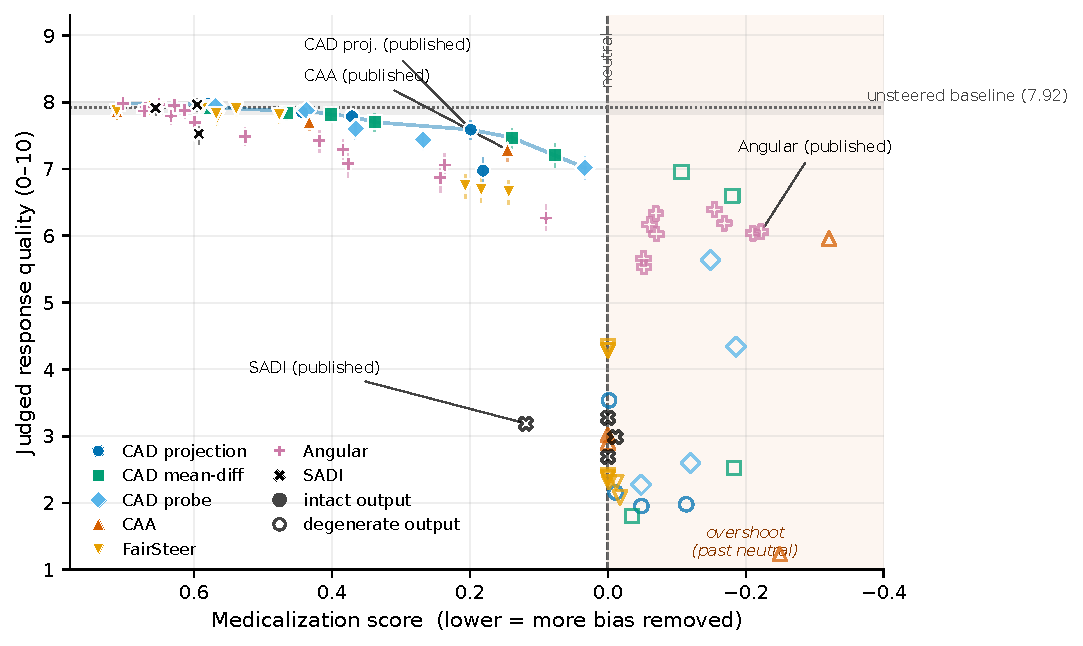
\includegraphics[width=\linewidth]{figure-01-quality-debiasing-frontier.pdf}
\caption{Judged quality against medicalization for 87 sweep points, $n{=}250$ responses
each. Filled markers are intact output, hollow markers are degenerate by the criterion
in Section~\ref{sec:frontier}, which uses text properties and not the quality score.
Error bars are bootstrap $95\%$ confidence intervals on the mean quality. The grey band
is the unsteered reference, $\pm 2$ standard deviations across ten no-steer points. The
shaded region past neutral marks responses that withhold medical information, which is
not an improvement. The blue line is the Pareto front over intact points.}
\label{fig:frontier}
\end{figure}

The Pareto front over intact points holds twelve configurations, ten of them CAD
operators. Restricting to points that remove at least half the baseline medicalization,
all four surviving front configurations are CAD: the probe at $\alpha{=}9$, the
mean-difference operator at $\alpha{=}8$ and $\alpha{=}7$, and the projection at
$\alpha{=}1$. No baseline method reaches that region of the plot without degenerating.

At matched strength the projection also scored above CAA in this sweep, by $0.30$
$[0.07, 0.53]$. That difference does not survive the held-out test
(Section~\ref{sec:confirm}), and we do not rely on it.

\subsection{Collapse is a threshold, and the published settings sit close to it}

Figure~\ref{fig:collapse}(a) in the appendix sweeps steering strength for each method. Quality holds
close to the unsteered reference and then falls steeply over a narrow range of
strengths. The fall is not gradual in any of them.


Raw strengths do not compare across methods, since each parameterises its intervention
differently. What does compare is the margin between the setting an author recommends
and the setting at which the method breaks. Taking the breaking point as the first
strength whose mean quality falls below $6.0$, that margin is $3.0\times$ for the CAD
projection, $2.0\times$ for CAA and for FairSteer, $1.9\times$ for the CAD
mean-difference operator, $1.2\times$ for the CAD probe, and $1.0\times$ for SADI.

SADI's published setting is its breaking point. At $s{=}5$ it scores $7.5$ on quality
and removes little bias; at $s{=}10$, the value its authors report, quality is $3.2$.
There is no intermediate setting in the published sweep at which the method both works
and leaves the text intact.

A wider margin is not immunity. The CAD projection is flagged degenerate from
$\alpha{=}3$, where $70\%$ of its responses become unparseable, and at $\alpha{=}5$ it
returns 75 empty responses out of 250. Every method here has a range in which it works
and a point past which it destroys the output. What separates them is how much room
sits between that point and the strength needed to remove the bias.

This also explains why the leaderboard inverts the ranking. Methods are tuned to
maximise the target metric, and the target metric keeps rewarding larger steering
strengths past the point where the text breaks, because broken text contains neither
medical nor professional vocabulary and the log-odds contrast
\citep{monroe2008fightin} goes to zero. The degeneration modes themselves are familiar
from open-ended generation \citep{welleck-etal-2019-neural}; what is new here is that a
fairness metric scores them as success.

\subsection{A second architecture}

On Qwen2.5-7B the projection operator reaches
$d{=}0.392$ at $\alpha{=}1$ with no degenerate output, and collapses at $\alpha{=}2$
rather than the $\alpha{=}3$ we observe for Llama-3.1-8B. The operating window is
narrower on Qwen, and the threshold structure of Figure~\ref{fig:collapse} replicates
with a different threshold.

\paragraph{Scope.} The sweep draws a separate 250-prompt subset per method and fits every
method on a pool that contains its evaluation prompts, so it supports the shape of the
curve and the ordering rather than paired effect sizes. Section~\ref{sec:confirm} removes
both limitations.

% Section 5: the pre-registered frozen-set test (E1 + amendment A4).
% Every number is from analysis-output/e1/e1_scores.json, written by e1_analysis.py from
% results/e1/ (evidence commits 370fe66 and ac8a93e). Pre-registration and deviations:
% claims/PREREG_E1_frozen_eval.md; verdicts: claims/E1_RESULTS.md.
\section{A pre-registered test on held-out questions}
\label{sec:confirm}

The sweep in Section~\ref{sec:frontier} was exploratory. Its settings were chosen after
earlier results were seen, every method was fit on the same pool its 250 evaluation
prompts came from, each method drew its own evaluation prompts, and intervals were
computed over responses although AccessEval's pairs are nested: each question appears
with several disability categories, and the dataset lists every question twice. Before
generating anything further we wrote down predictions, falsifiers and stopping gates, and
ran them on one frozen evaluation set (Appendix~\ref{app:e1}).

\paragraph{Design.} The frozen set holds five disability variants of each of 50
questions, 250 items. Every method is fit only on the 633 distinct pairs of the other 96
questions; as a leak control, the projection and CAA are also fit on the full pool. Each
baseline runs at its published setting, the projection at $\alpha{=}1$ with $k{=}40$.
Quality is scored by two judges from different model families, Llama-3.1-8B-Instruct and
Qwen2.5-7B-Instruct, with the same rubric; they agree per item at Spearman
$\rho{=}0.64$. Intervals are bootstrapped over the 50 questions. Three unsteered seeds
agree to within $0.013$ in mean medicalization, and the degeneracy flags are those of
Section~\ref{sec:frontier}.

\begin{table}[t]
\centering\footnotesize
\setlength{\tabcolsep}{3.2pt}
\begin{tabular}{@{}lrrrr@{}}
\toprule
& \multicolumn{1}{c}{$d$ \scriptsize[95\% CI]} & $\Delta$Med & \multicolumn{2}{c}{$\Delta$Quality} \\
\cmidrule(l){4-5}
& & \% & Llama & Qwen \\
\midrule
\multicolumn{5}{@{}l}{\textit{Prompting only}} \\
Minimal prompt & $-0.04$ \scriptsize$[-.14,.06]$ & $-8$ & $-0.03$ & $-0.03$ \\
Explicit prompt & $0.06$ \scriptsize$[-.02,.15]$ & $13$ & $+0.01$ & $+0.07$ \\
\midrule
\multicolumn{5}{@{}l}{\textit{Steering, intact output}} \\
CAD projection & $0.34$ \scriptsize$[.21,.48]$ & $66$ & $\mathbf{-0.59}$ & $-0.23$ \\
CAD mean-diff.\ $\alpha{=}7$ & $0.43$ \scriptsize$[.32,.56]$ & $91$ & $-0.72$ & $-0.24$ \\
CAA & $0.37$ \scriptsize$[.24,.51]$ & $77$ & $-0.80$ & $-0.30$ \\
FairSteer & $0.28$ \scriptsize$[.15,.42]$ & $59$ & $-1.31$ & $-0.61$ \\
LEACE, rank 40 & $0.17$ \scriptsize$[.05,.29]$ & $37$ & $-0.43$ & $-0.23$ \\
\midrule
\multicolumn{5}{@{}l}{\textit{Prompt and steering combined}} \\
Explicit + projection & $\mathbf{0.51}$ \scriptsize$[.37,.66]$ & $\mathbf{97}$ & $-0.70$ & $\mathbf{-0.20}$ \\
\midrule
\multicolumn{5}{@{}l}{\textit{Degenerate output}} \\
SADI $s{=}10$ & $0.30$ \scriptsize$[.10,.53]$ & $49$ & $-3.93$ & $-2.38$ \\
Angular $150^\circ$ & $0.74$ \scriptsize$[.58,.95]$ & $143$ & $-2.07$ & $-0.66$ \\
\bottomrule
\end{tabular}
\caption{The frozen-set test: 250 items from 50 held-out questions, one shared
unsteered reference (medicalization $0.597$; quality $7.85$ Llama, $6.70$ Qwen).
$\Delta$Med above 100 means the model was pushed past neutral. Bold marks the best value
among intact arms that remove at least half the medicalization. Every arm is in Appendix~\ref{app:e1}.}
\label{tab:e1}
\end{table}

\begin{figure*}[t]
\centering
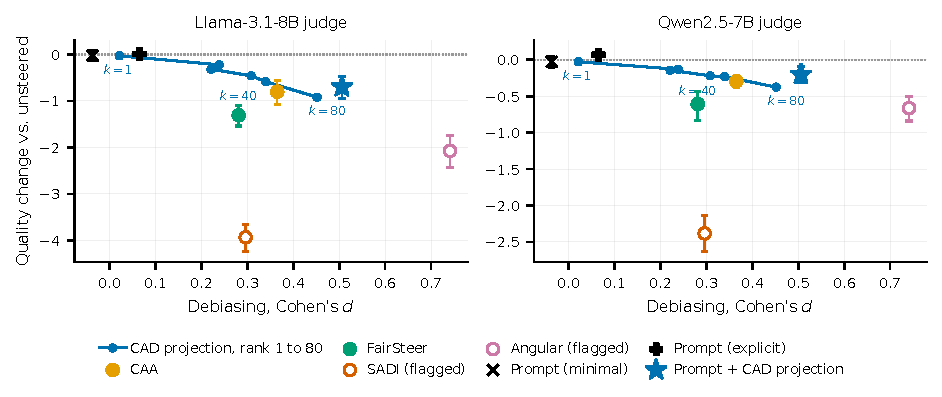
\includegraphics[width=\textwidth]{figure-02-e1-frozen-set.pdf}
\caption{Every arm of the frozen-set test under both judges. Horizontal: debiasing; vertical:
change in judged quality against the unsteered reference. Lines join strengths or ranks of
one operator. Hollow markers are flagged degenerate from the text alone. Error bars are
$95\%$ intervals over the 50 questions. The two judges differ in scale but agree on the
ordering, and the highest-$d$ point in both panels is broken output.}
\label{fig:e1}
\end{figure*}

\paragraph{The highest scores still belong to broken output.} Angular Steering has the
largest effect size of any arm, $d{=}0.74$, by pushing medicalization past neutral to
$-0.26$, and it loses $2.07$ points of judged quality. SADI at its published setting
scores exactly zero on $58\%$ of responses, and a fifth of its responses cannot be parsed
by the judge. Ordered by quality loss, the five published methods fall in the same order
under both judges, as pre-registered: SADI, Angular, FairSteer, CAA, and the projection.
Ordered by $d$, Angular comes first and SADI ranks above FairSteer.

\paragraph{What did not replicate.} The sweep suggested that the projection loses less
quality than CAA at comparable debiasing. On held-out questions the paired difference is
$+0.22$ $[-0.12, 0.57]$ under the Llama judge and $+0.06$ $[-0.03, 0.15]$ under Qwen, and
debiasing is $0.34$ against $0.37$. The point estimates favour the projection and the
intervals include zero, so we treat the two as equally intact at matched debiasing. The
earlier significant result (Appendix~\ref{app:earlier}) computed intervals over
responses, treating variants of one question as independent, which is the error
Section~\ref{sec:geometry} finds in spectral estimates. The leak did not matter: fitting
on the full pool, evaluation questions included, raises $d$ by $0.004$ for the projection
and $0.001$ for CAA.

\subsection{Prompting does not remove the bias, and combines with steering}
\label{sec:prompting}

Prompting outperforms representation steering on AxBench \citep{wu2025axbench}, so we
added two system prompts, worded before any prompted output existed. The minimal one asks
the model to mention a disability only where it changes the answer; the explicit one
tells it not to assume a disabled person needs medical treatment, diagnosis or therapy.
Neither costs quality, and neither removes much bias: the minimal prompt leaves
medicalization where it was ($d{=}{-}0.04$) and the explicit one removes $13\%$
($d{=}0.06$). The projection removes more than the explicit prompt by $0.28$
$[0.14, 0.44]$. Concept removal is where \citet{macocco2026tradeoff} also find prompting
weakest.

The two combine. With the explicit prompt in place, the projection reaches $d{=}0.51$
$[0.37, 0.66]$ and removes $97\%$ of medicalization with no flagged output, $0.08$ to
$0.26$ more than the projection alone, at a quality cost of $0.70$ (Llama) and $0.20$
(Qwen). No intact arm reaches a higher $d$ (Figure~\ref{fig:e1}). The directions were fit
under the default prompt and still act under the new one.

\subsection{What rank does}
\label{sec:rank}

Removing more directions removes more medicalization and costs more quality
(Figure~\ref{fig:e1}, dark blue line). The projection goes from $d{=}0.02$ at rank 1 to
$0.34$ at rank 40 and $0.45$ at rank 80, while the quality change under the Llama judge
goes from $-0.03$ to $-0.59$ to $-0.92$. Rank-$k$ LEACE \citep{belrose2023leace}, erasing
the same top-$k$ coordinates with whitening, shows the same trend more weakly: $0.01$,
$0.17$ $[0.05, 0.29]$ and $0.30$. Its rank-1 and rank-40 intervals overlap by $0.03$, so
the pre-registered prediction that rank 40 beats rank 1 for both operators fails on
LEACE. Removing the single direction of a supervised probe gives $d{=}0.08$
$[-0.01, 0.18]$: one well-chosen direction, removed, does not reproduce the effect of
forty.

What survives is narrower than a claim about the dimensionality of the bias. A single
removed direction does little, and beyond that rank behaves like a strength setting with
the same trade-off every other strength parameter shows. Section~\ref{sec:geometry}
explains why the rank cannot instead be read off the data.

\section{Measured bias dimensionality is a property of the contrast set}
\label{sec:geometry}

Section~\ref{sec:rank} found that intervention rank trades debiasing against quality. A
natural next step is to estimate, for a given behaviour, how many dimensions its
representation occupies, and to set the rank from that estimate, as our own pipeline
originally did.

The usual estimator is the singular value spectrum of a stack of contrastive
activation differences: collect pairs of prompts differing only in the
attribute of interest, take the difference of their activations, and read off
the top explained-variance ratio ($\mathrm{EVR}_1$) or the rank needed to
reach some fraction of the variance ($k@80\%$). Low $\mathrm{EVR}_1$ is read
as a diffuse behaviour needing many directions; high $\mathrm{EVR}_1$ as a
concentrated one that a single vector can address.

We ran four controls on this estimator. All four use the AccessEval
contrastive pool of 2{,}083 pairs on Llama-3.1-8B-Instruct, and all four
indicate that $\mathrm{EVR}_1$ and $k@80\%$ report properties of the
contrastive set rather than of the bias.

\begin{table}[t]
\centering
\small
\begin{tabular}{lrr}
\toprule
Contrast set ($n{=}13$, L21) & $\mathrm{EVR}_1$ & $k@80\%$ \\
\midrule
Heterogeneous (any query)      & $22.1\%$ & $7.0$ \\
Single category                & $22.3\%$ & $7.0$ \\
Single domain                  & $27.1\%$ & $5.9$ \\
5 base queries only            & $44.2\%$ & $3.1$ \\
2 base queries only            & $\mathbf{76.1\%}$ & $\mathbf{1.7}$ \\
\midrule
\multicolumn{3}{l}{\textit{Paper's reported Target A (L4+L15, $n{=}13$)}} \\
\quad reported profile         & $67.9\%$ & $2$ \\
\bottomrule
\end{tabular}
\caption{Holding the number of contrastive pairs fixed at 13 and varying only how many
distinct base queries they are drawn from. Means over 40 draws. The $95\%$ intervals are
$[17.8, 28.4]$ for the heterogeneous row and $[62.0, 87.5]$ for two base queries. The
profile the paper reports for DiscrimEval Target A falls inside the latter interval and
matches its rank. The effect replicates at L14, where the same contrast runs from
$22.9\%$ $[18.1, 28.6]$ to $69.4\%$ $[54.3, 80.4]$.}
\label{tab:homogeneity}
\end{table}

\paragraph{Prompt diversity moves the estimate more than anything else.}
We fix the number of pairs at $n{=}13$ and vary only how many distinct base
queries those pairs are drawn from (Table~\ref{tab:homogeneity}). Drawn from
the whole pool, $\mathrm{EVR}_1$ is $22.1\%$ with $k@80\%{=}7.0$. Restricted
to two base queries, the same benchmark at the same layer gives
$\mathrm{EVR}_1{=}76.1\%$ $[62\%, 87\%]$ with $k@80\%{=}1.7$. The effect
replicates at L14 ($22.9\%$ to $69.4\%$ $[54\%, 80\%]$). A benchmark
described as forty-dimensional produces a near-rank-1 spectrum when its
prompts are made homogeneous.

\paragraph{Three further controls agree.} Sampling 13 pairs by drawing whole base
queries rather than uniformly moves $\mathrm{EVR}_1$ from $21.5\%$ to $72.2\%$ on the
same data at the same layer. A null built by permuting the pairing, which destroys the
contrast while preserving both marginals, is \emph{higher} than the real data at
$n{=}13$ ($26.2\%$ against $21.5\%$) and separates from it only above $n \approx 250$,
so a concentration estimated from a dozen pairs is consistent with no contrastive
structure at all. And resampling pairs directly gives $k@80\%{=}40$ $[40, 41]$ where
resampling the 146 distinct questions gives $30.1$ $[27, 33]$, intervals that do not
overlap, so treating nested pairs as independent is not merely over-precise.
Appendix~\ref{app:controls} gives all three in full. The held-out test supplied a fifth
instance unprompted: the rank reaching $80\%$ of the variance is 33 and 36 at the two
layers when fit on the 633 held-out pairs, and 42 and 49 on the full 1{,}044, for the
same bias at the same layers.

\paragraph{What this means for the diagnostic.} Taken together, these
controls remove the basis for using $\mathrm{EVR}_1$ to prescribe an
intervention rank. Two benchmarks can differ in reported dimensionality
because one varies a single template while the other spans nine categories
and six domains, with no difference in the underlying bias. We had read the
same signal as evidence that bias geometry varies by bias type, and it does
not follow.

One earlier observation reads differently in this light. The first singular direction is
close to orthogonal to a trained probe for the same attribute ($\cos{=}{-}0.001$ at L21),
so the top of the spectrum is not measuring the bias either.

% PORTED from paper_aaai2027/main.tex Related Work, with two changes:
%  - removed "CAD predicts each failure from the singular value spectrum before any
%    steered generation" and the EVR->alpha prescription framing (falsified, Sec 5)
%  - narrowed the novelty claim: HiDRA / SAE-SSV / CAS-BiPO do read structure off
%    contrastive activations, so the gap is not that nobody looks at the subspace.
% TODO before submission: fetch BibTeX for HiDRA (arXiv 2606.15092), SAE-SSV
% (arXiv 2505.16188, EMNLP 2025) and CAS-BiPO (2026.findings-eacl.57) and cite them in
% the marked sentence. Do not cite until the entries are verified.
\section{Related work}
\label{sec:related}

\paragraph{Activation steering for bias.} Activation Addition
\citep{turner2023activation} and CAA \citep{rimsky2024steering} compute mean-difference
vectors from contrastive pairs and add them at inference. FairSteer
\citep{li2025fairsteer} adds a classifier gate, and Shifting Perspectives
\citep{siddique2025shifting} trains per-axis PCA vectors from BBQ. Methods that go
beyond a single direction commit to a structure without checking it: SADI
\citep{wang2025sadi} and Angular Steering \citep{vu2025angular} both reach high
target-metric scores at settings that damage the text, and RePS \citep{wu2025reps}
requires training-time gradients. Our comparison differs in what it holds fixed. We
sweep each method across its published range and score response quality at every point,
which is what separates a method that removed the bias from one that removed the answer.

\paragraph{Reading structure off contrastive activations.} Closest to our decomposition
is Representation Engineering's Linear Artificial Tomography \citep{zou2023representation},
which takes principal components of representation \textit{differences} over contrastive
pairs. Distributed Alignment Search \citep{geiger2024das} learns a rotated basis aligning
causal variables with subspaces, and sparse autoencoders \citep{cunningham2024sae} learn
an overcomplete monosemantic basis. Several recent bias-steering methods go further and
set the rank or the target subspace of an intervention from statistics of that
decomposition.% TODO: cite HiDRA, SAE-SSV, CAS-BiPO here once BibTeX is verified.
Section~\ref{sec:geometry} is addressed to that step specifically. We do not claim these
methods are wrong; we show that the statistic they read is sensitive to how the
contrastive set was assembled, which means it cannot by itself distinguish one bias from
another. The practical recommendation there, reporting the number of independent base
prompts alongside the number of pairs, is cheap enough to apply to any of them.

\paragraph{Subspace methods for fairness.} Earlier subspace work debiases static word
embeddings \citep{bolukbasi2016man, ravfogel2020null} or learns closed-form erasure
projections from training data \citep{belrose2023leace}. We apply the same family of
operator to activation differences at inference time, and Section~\ref{sec:rank} uses
LEACE directly as the control that isolates rank.

\paragraph{Degenerate text and its measurement.} Repetition and collapse under
open-ended generation are well documented \citep{welleck-etal-2019-neural}. The
observation in this paper is not that steering can degrade text, which is expected, but
that a fairness metric built on vocabulary absence scores that degradation as success,
and that the methods sitting at the top of the leaderboard are the ones it affects most.

\section{Conclusion}
\label{sec:conclusion}

A model asked about exercise by a user who mentions a disability answers a different
question, one about risk and supervision. Removing that behaviour at inference time is a
reasonable goal, and the field measures progress toward it with a metric that counts the
clinical vocabulary the model stops producing.

That metric cannot tell the difference between a model that stopped medicalizing and a
model that stopped writing. We found three methods sitting at settings where it reports
success and the responses are corrupted, looped, or truncated, and the failure modes
differ enough that no single filter on emptiness, length or uniqueness catches them all.
The method with the lowest score in our comparison is the one that damages the output
most.

Measuring quality alongside the target metric changes the ranking and leaves a usable
picture: a narrow band of configurations that reduce medicalization while leaving the
text intact, occupied almost entirely by multi-rank projection at the operating point its
rank prescribes. That rank matters is a separate and simpler claim than the one we set
out to make, and it survives the control experiments that the stronger claim does not.

The practical recommendation is small and cheap. Report a quality measure beside the
target metric, since a vocabulary-absence score is satisfied by absence of any kind. And
report the number of independent base prompts alongside the number of contrastive pairs,
since the spectral statistics read off those pairs move further under a change of prompt
diversity than under a change of bias.


% ---- everything below this line is OUTSIDE the 8-page content budget ----
\section*{Limitations}
\label{sec:limitations}

\paragraph{Scope.} All results use one benchmark, AccessEval, in English, on 7B- and
8B-parameter instruction-tuned models. We do not claim the thresholds or the ordering
transfer to other metrics, demographic axes or model scales.

\paragraph{Judges.} Quality is scored by two language-model judges, not by people. The
judges agree on the ordering and differ in scale, and Llama-3.1-8B scores outputs of its
own family.

\paragraph{What the held-out test covers.} It evaluates each baseline at its published
setting and the projection at one strength, not the full frontier. Two prompts were
tested, worded once and not tuned, and a better prompt may remove more bias. The combined
arm uses one prompt and one rank.

Appendices~\ref{app:judge}--\ref{app:e1} give the supporting detail.


\bibliography{custom}

\appendix
% APPENDIX. Does not count toward the 8-page content limit (verified from the ARR CFP).
% Everything here is reproducible from the artifacts named in each section.
% TODO still to port from paper_aaai2027/main.tex supplementary:
%   - Unfiltered evaluation on n=250
%   - Per-disability-category stratification
%   - Mechanistic accounts of baselines (propagation metrics)
%   - Phase 1 vocabulary threshold robustness
%   - Why SVD, not PCA or ICA
%   - Qualitative examples (6 prompt types) and the cross-method comparison table

\section{Judge protocol}
\label{app:judge}

Responses are scored by Llama-3.1-8B-Instruct against a ten-point accessibility rubric,
with \texttt{temperature}$=0.1$, seed 42, and responses truncated to 2{,}000 characters.
The judge is asked for a line of the form \texttt{Overall Score: X/10}, and a response
whose output cannot be parsed, or which is empty, receives $5.0$.

That default deserves scrutiny, since $5.0$ is also a plausible middling score. Across
the 2{,}500 unsteered responses, none receives exactly $5.0$. In this run the value marks
failure rather than mediocrity. Recoding every $5.0$ to zero moves SADI from $3.19$ to
$1.37$, because $36.4\%$ of its responses are unparseable, and moves no other method by
more than $0.05$. The default therefore understates the collapse, and every quality drop
reported in the main text is conservative.

Scoring is deduplicated by response hash: 21{,}750 responses reduce to 19{,}888 unique
texts, each scored once.

\section{Statistical procedures}
\label{app:stats}

The unit of analysis is one sweep point, meaning one method at one configuration, with
$n{=}250$ responses. Intervals on a mean judge score are percentile bootstrap intervals
over 2{,}000 resamples of the 250 responses, seed 42.

Judge scores take eight distinct values and are strongly left-skewed at degenerate
points, so normality fails and we use the Mann-Whitney $U$ test with rank-biserial
correlation as the effect size rather than a $t$-test. Comparisons of the five published
operating points against the pooled unsteered baseline are Holm-corrected across those
five tests. The Pareto front is a descriptive geometric construction and carries no
$p$-value.

Responses within a sweep point come from different prompts and are treated as
independent. The same prompt recurs across sweep points, so comparisons between points
are not strictly independent; we report them as unpaired regardless, which widens the
intervals rather than narrowing them.

Two consequences of the measurement are worth stating. The judge emits eight distinct
values, so it does not grade fine gradations within a single response; at $n{=}250$ the
resulting interval on a point mean has a median half-width of $0.18$. And our CAD runner
records medicalization in aggregate rather than per response, so the CAD points in
Figure~\ref{fig:frontier} carry no interval on the horizontal axis.

The unpaired and matched designs agree on the comparison they share. The frontier gives
$+0.30$ with interval $[0.07, 0.53]$ for the projection against CAA; the matched-item
test in Section~\ref{sec:paired} gives $+0.35$ with $[0.18, 0.53]$.

\section{Sensitivity of the degeneracy criterion}
\label{app:thresholds}

The criterion in Section~\ref{sec:frontier} uses three cut-offs: uniqueness below
$0.50$, parse-failure rate above $0.10$, and medicalization below $-0.05$. These are
conventional rather than derived, so we varied all three. Across the 27 combinations of
$\{0.3, 0.5, 0.7\} \times \{0.05, 0.10, 0.20\} \times \{-0.10, -0.05, 0\}$ the Pareto
front holds the same twelve configurations, ten of them CAD operators, and the same four
configurations reaching at least half the baseline reduction.

Relative to applying no criterion at all, flagging removes exactly one configuration
from the front, FairSteer at $\alpha{=}8$, which reaches medicalization $0.000$ with 68
of its 250 responses distinct.

\section{Contrast-set controls in full}
\label{app:controls}

Section~\ref{sec:geometry} reports the homogeneity ladder in the main text and summarises
three further controls. This section gives those three, all on the AccessEval contrastive
pool of 2{,}083 pairs on Llama-3.1-8B-Instruct.

\paragraph{Cluster versus pair sampling.} AccessEval expands 234 questions, each listed twice, into
4{,}164 pairs by substituting nine disability categories into templated queries, so pairs are
nested within base queries. Sampling 13 pairs uniformly gives $\mathrm{EVR}_1{=}21.5\%$;
sampling 13 pairs by drawing whole base queries gives $72.2\%$. Same data, same $n$, same
layer, a $3.4$-fold swing from the sampling structure alone. The gap closes as $n$ grows:
$15.6\%$ against $40.4\%$ at $n{\approx}30$, $11.1\%$ against $14.1\%$ at $n{\approx}250$,
and $10.4\%$ against $10.8\%$ at $n{\approx}1000$.

\paragraph{A permuted-pairing null.} We match each clean activation to a different
corrupted one, destroying the contrast while preserving both marginals. At $n{=}13$ the
real data give $\mathrm{EVR}_1{=}21.5\%$ and the null gives $26.2\%$, so the null is
higher. The two curves separate only above $n \approx 250$
(Figure~\ref{fig:controls}). Any concentration estimated from a dozen pairs is consistent
with no contrastive structure at all, which is the regime the reported Target A profile
sits in.

\paragraph{Cluster bootstrap.} Resampling the 2{,}083 pairs of the filtered pool
directly gives $k@80\%{=}40$ with a $95\%$ interval of $[40, 41]$. The pairs are not
independent: every pair is one of several disability variants of a question, and AccessEval
lists each question twice, so the pool comes from only 146 distinct questions. Resampling
those 146 questions instead gives $k@80\%{=}30.1$ $[27, 33]$ at L21, $28.2$ $[26, 30]$ at
L14, and $10.2$ $[9, 11]$ at L0 (150 resamples each). The pair-level and question-level
intervals do not overlap at L21, so the pair-level procedure is biased as well as
over-precise.

\begin{figure*}[t]
\centering
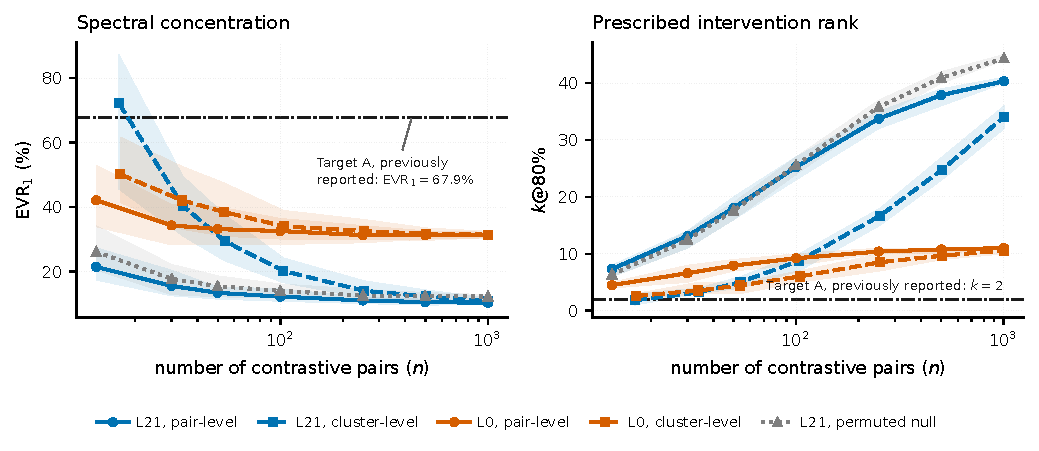
\includegraphics[width=\textwidth]{figure-03-contrast-set-controls.pdf}
\caption{Spectral concentration (left) and prescribed rank (right) against the number of
contrastive pairs, on AccessEval. Solid lines sample pairs uniformly; dashed lines sample
whole base queries; the dotted grey line is a null built by permuting the pairing, which
destroys the contrast while preserving both marginals. Bands are $95\%$ intervals over 40
draws. Below $n \approx 250$ the real data and the null are not separated, so spectra
estimated from a dozen pairs carry no contrastive signal. The dash-dotted line marks the
profile the paper reports for Target A.}
\label{fig:controls}
\end{figure*}


\section{Reproduction}
\label{app:repro}

Generation and judging ran on a single A100 80GB. The five sweeps took approximately
eleven GPU-hours in total and the judging pass approximately three. The diagnostic
itself is cheap next to either: collecting activations over the contrastive pairs is one
forward pass, and the truncated SVD of the resulting $n \times d$ difference matrix takes
seconds. The projection is then applied at $\alpha{=}1$ with no strength search, which is
the practical difference from the additive baselines, each of which requires a
layer-by-strength grid where every cell is a full generation-and-scoring pass.

\section{Complete sweep}
\label{app:sweep}

Tables~\ref{tab:allsweep1}--\ref{tab:allsweep3} list every sweep point behind
Figure~\ref{fig:frontier}: 87 configurations, $n{=}250$ responses each, 21{,}750
responses in total. Quality is the mean judge score with a percentile bootstrap $95\%$
interval over 2{,}000 resamples. ``Uniq'' is the fraction of the 250 responses that are
distinct and ``Fail'' the fraction the judge could not parse. A point is marked
degenerate ($\bullet$) when uniqueness falls below $0.50$, the failure rate exceeds
$0.10$, or medicalization falls below $-0.05$.

\begin{table*}[t]
\centering\small
\begin{tabular}{llrrrrc}
\toprule
Method & Configuration & Med. & Quality \scriptsize[95\% CI] & Uniq & Fail & Deg. \\
\midrule
Angular & max\_sim\_L23/mode\_0/angle\_150 & $-0.222$ & $6.06$ \scriptsize$[5.86,\,6.24]$ & $1.00$ & $0.01$ & $\bullet$ \\
Angular & max\_sim\_L23/mode\_1/angle\_150 & $-0.210$ & $6.04$ \scriptsize$[5.83,\,6.23]$ & $1.00$ & $0.01$ & $\bullet$ \\
Angular & max\_sim\_L23/mode\_0/angle\_120 & $-0.169$ & $6.19$ \scriptsize$[6.00,\,6.38]$ & $1.00$ & $0.00$ & $\bullet$ \\
Angular & max\_sim\_L23/mode\_1/angle\_120 & $-0.154$ & $6.39$ \scriptsize$[6.22,\,6.58]$ & $1.00$ & $0.00$ & $\bullet$ \\
Angular & max\_sim\_L23/mode\_0/angle\_180 & $-0.071$ & $6.02$ \scriptsize$[5.82,\,6.21]$ & $1.00$ & $0.02$ & $\bullet$ \\
Angular & max\_sim\_L23/mode\_1/angle\_180 & $-0.070$ & $6.34$ \scriptsize$[6.15,\,6.52]$ & $1.00$ & $0.01$ & $\bullet$ \\
Angular & max\_norm\_L31/mode\_0/angle\_150 & $-0.060$ & $6.17$ \scriptsize$[5.98,\,6.35]$ & $1.00$ & $0.00$ & $\bullet$ \\
Angular & max\_norm\_L31/mode\_0/angle\_180 & $-0.052$ & $5.53$ \scriptsize$[5.32,\,5.74]$ & $1.00$ & $0.00$ & $\bullet$ \\
Angular & max\_norm\_L31/mode\_1/angle\_180 & $-0.052$ & $5.66$ \scriptsize$[5.44,\,5.86]$ & $1.00$ & $0.00$ & $\bullet$ \\
Angular & max\_norm\_L31/mode\_1/angle\_150 & $0.090$ & $6.26$ \scriptsize$[6.07,\,6.46]$ & $1.00$ & $0.00$ &  \\
Angular & max\_norm\_L31/mode\_1/angle\_270 & $0.237$ & $7.06$ \scriptsize$[6.86,\,7.23]$ & $1.00$ & $0.01$ &  \\
Angular & max\_norm\_L31/mode\_0/angle\_270 & $0.243$ & $6.87$ \scriptsize$[6.65,\,7.06]$ & $1.00$ & $0.00$ &  \\
Angular & max\_sim\_L23/mode\_0/angle\_270 & $0.377$ & $7.08$ \scriptsize$[6.87,\,7.26]$ & $1.00$ & $0.00$ &  \\
Angular & max\_norm\_L31/mode\_0/angle\_120 & $0.384$ & $7.29$ \scriptsize$[7.12,\,7.45]$ & $1.00$ & $0.00$ &  \\
Angular & max\_sim\_L23/mode\_1/angle\_270 & $0.418$ & $7.42$ \scriptsize$[7.25,\,7.58]$ & $1.00$ & $0.00$ &  \\
Angular & max\_norm\_L31/mode\_1/angle\_120 & $0.526$ & $7.49$ \scriptsize$[7.35,\,7.62]$ & $1.00$ & $0.00$ &  \\
Angular & max\_sim\_L23/mode\_0/angle\_60 & $0.599$ & $7.70$ \scriptsize$[7.58,\,7.80]$ & $1.00$ & $0.00$ &  \\
Angular & max\_sim\_L23/mode\_0/angle\_0 & $0.614$ & $7.88$ \scriptsize$[7.76,\,7.98]$ & $1.00$ & $0.00$ &  \\
Angular & max\_norm\_L31/mode\_1/angle\_0 & $0.629$ & $7.95$ \scriptsize$[7.84,\,8.05]$ & $1.00$ & $0.00$ &  \\
Angular & max\_sim\_L23/mode\_1/angle\_60 & $0.633$ & $7.79$ \scriptsize$[7.66,\,7.91]$ & $1.00$ & $0.00$ &  \\
Angular & max\_norm\_L31/mode\_1/angle\_60 & $0.651$ & $7.97$ \scriptsize$[7.87,\,8.06]$ & $1.00$ & $0.00$ &  \\
Angular & max\_norm\_L31/mode\_0/angle\_0 & $0.670$ & $7.92$ \scriptsize$[7.82,\,8.00]$ & $1.00$ & $0.00$ &  \\
Angular & max\_norm\_L31/mode\_0/angle\_60 & $0.672$ & $7.87$ \scriptsize$[7.78,\,7.95]$ & $1.00$ & $0.00$ &  \\
Angular & max\_sim\_L23/mode\_1/angle\_0 & $0.703$ & $7.98$ \scriptsize$[7.87,\,8.07]$ & $1.00$ & $0.00$ &  \\
CAA & L14/alpha\_2.0 & $-0.321$ & $5.96$ \scriptsize$[5.74,\,6.17]$ & $1.00$ & $0.00$ & $\bullet$ \\
CAA & L14/alpha\_4.0 & $-0.249$ & $1.24$ \scriptsize$[1.06,\,1.40]$ & $1.00$ & $0.05$ & $\bullet$ \\
CAA & L14/alpha\_6.0 & $0.000$ & $3.02$ \scriptsize$[2.72,\,3.32]$ & $0.99$ & $0.60$ & $\bullet$ \\
CAA & L14/alpha\_8.0 & $0.000$ & $2.90$ \scriptsize$[2.62,\,3.20]$ & $0.84$ & $0.56$ & $\bullet$ \\
CAA & L14/alpha\_1.0 & $0.146$ & $7.29$ \scriptsize$[7.11,\,7.46]$ & $1.00$ & $0.00$ &  \\
CAA & L14/alpha\_0.5 & $0.433$ & $7.70$ \scriptsize$[7.58,\,7.82]$ & $1.00$ & $0.00$ &  \\
\bottomrule
\end{tabular}
\caption{All sweep points, part 1 of 3.}
\label{tab:allsweep1}
\end{table*}

\begin{table*}[t]
\centering\small
\begin{tabular}{llrrrrc}
\toprule
Method & Configuration & Med. & Quality \scriptsize[95\% CI] & Uniq & Fail & Deg. \\
\midrule
CAA & L14/alpha\_0.0 & $0.712$ & $7.87$ \scriptsize$[7.74,\,7.98]$ & $1.00$ & $0.00$ &  \\
CAD mean-diff & alpha15.0 & $-0.183$ & $2.52$ \scriptsize$[2.28,\,2.77]$ & $1.00$ & $0.28$ & $\bullet$ \\
CAD mean-diff & alpha10.0 & $-0.180$ & $6.60$ \scriptsize$[6.41,\,6.80]$ & $1.00$ & $0.00$ & $\bullet$ \\
CAD mean-diff & alpha9.0 & $-0.107$ & $6.96$ \scriptsize$[6.78,\,7.13]$ & $1.00$ & $0.00$ & $\bullet$ \\
CAD mean-diff & alpha20.0 & $-0.035$ & $1.81$ \scriptsize$[1.52,\,2.10]$ & $0.99$ & $0.30$ & $\bullet$ \\
CAD mean-diff & alpha8.0 & $0.077$ & $7.20$ \scriptsize$[7.03,\,7.38]$ & $1.00$ & $0.00$ &  \\
CAD mean-diff & alpha7.0 & $0.139$ & $7.47$ \scriptsize$[7.31,\,7.61]$ & $1.00$ & $0.00$ &  \\
CAD mean-diff & alpha5.0 & $0.338$ & $7.70$ \scriptsize$[7.56,\,7.83]$ & $1.00$ & $0.00$ &  \\
CAD mean-diff & alpha3.0 & $0.402$ & $7.82$ \scriptsize$[7.70,\,7.92]$ & $1.00$ & $0.00$ &  \\
CAD mean-diff & alpha2.0 & $0.466$ & $7.84$ \scriptsize$[7.72,\,7.95]$ & $1.00$ & $0.00$ &  \\
CAD mean-diff & alpha1.0 & $0.583$ & $7.92$ \scriptsize$[7.81,\,8.01]$ & $1.00$ & $0.00$ &  \\
CAD probe & alpha13.0 & $-0.186$ & $4.34$ \scriptsize$[4.11,\,4.57]$ & $1.00$ & $0.04$ & $\bullet$ \\
CAD probe & alpha11.0 & $-0.149$ & $5.64$ \scriptsize$[5.44,\,5.83]$ & $1.00$ & $0.02$ & $\bullet$ \\
CAD probe & alpha15.0 & $-0.120$ & $2.60$ \scriptsize$[2.37,\,2.83]$ & $0.99$ & $0.20$ & $\bullet$ \\
CAD probe & alpha17.0 & $-0.048$ & $2.27$ \scriptsize$[1.97,\,2.56]$ & $0.99$ & $0.38$ & $\bullet$ \\
CAD probe & alpha9.0 & $0.034$ & $7.02$ \scriptsize$[6.85,\,7.19]$ & $1.00$ & $0.00$ &  \\
CAD probe & alpha7.0 & $0.268$ & $7.44$ \scriptsize$[7.27,\,7.59]$ & $1.00$ & $0.00$ &  \\
CAD probe & alpha5.0 & $0.366$ & $7.60$ \scriptsize$[7.44,\,7.74]$ & $1.00$ & $0.00$ &  \\
CAD probe & alpha3.0 & $0.437$ & $7.87$ \scriptsize$[7.75,\,7.99]$ & $1.00$ & $0.00$ &  \\
CAD probe & alpha1.0 & $0.569$ & $7.94$ \scriptsize$[7.84,\,8.04]$ & $1.00$ & $0.00$ &  \\
CAD projection & alpha9.0 & $-0.114$ & $1.98$ \scriptsize$[1.66,\,2.29]$ & $0.94$ & $0.39$ & $\bullet$ \\
CAD projection & alpha7.0 & $-0.049$ & $1.95$ \scriptsize$[1.65,\,2.24]$ & $0.96$ & $0.38$ & $\bullet$ \\
CAD projection & alpha5.0 & $-0.011$ & $2.16$ \scriptsize$[1.86,\,2.43]$ & $0.80$ & $0.40$ & $\bullet$ \\
CAD projection & alpha3.0 & $-0.002$ & $3.54$ \scriptsize$[3.25,\,3.80]$ & $0.83$ & $0.70$ & $\bullet$ \\
CAD projection & alpha2.0 & $0.181$ & $6.98$ \scriptsize$[6.78,\,7.17]$ & $1.00$ & $0.00$ &  \\
CAD projection & alpha1.0 & $0.199$ & $7.59$ \scriptsize$[7.44,\,7.73]$ & $1.00$ & $0.01$ &  \\
CAD projection & alpha0.5 & $0.371$ & $7.79$ \scriptsize$[7.67,\,7.90]$ & $1.00$ & $0.01$ &  \\
CAD projection & alpha0.3 & $0.444$ & $7.85$ \scriptsize$[7.74,\,7.96]$ & $1.00$ & $0.00$ &  \\
CAD projection & alpha0.1 & $0.580$ & $7.97$ \scriptsize$[7.88,\,8.06]$ & $1.00$ & $0.00$ &  \\
FairSteer & L29/thresh\_0.7/alpha\_4.0 & $-0.018$ & $2.08$ \scriptsize$[1.80,\,2.38]$ & $0.97$ & $0.36$ & $\bullet$ \\
\bottomrule
\end{tabular}
\caption{All sweep points, part 2 of 3.}
\label{tab:allsweep2}
\end{table*}

\begin{table*}[t]
\centering\small
\begin{tabular}{llrrrrc}
\toprule
Method & Configuration & Med. & Quality \scriptsize[95\% CI] & Uniq & Fail & Deg. \\
\midrule
FairSteer & L29/thresh\_0.5/alpha\_4.0 & $-0.012$ & $2.31$ \scriptsize$[2.02,\,2.61]$ & $0.94$ & $0.38$ & $\bullet$ \\
FairSteer & L29/thresh\_0.3/alpha\_4.0 & $-0.002$ & $2.31$ \scriptsize$[2.02,\,2.62]$ & $0.95$ & $0.39$ & $\bullet$ \\
FairSteer & L29/thresh\_0.3/alpha\_6.0 & $0.000$ & $2.42$ \scriptsize$[2.12,\,2.73]$ & $0.30$ & $0.40$ & $\bullet$ \\
FairSteer & L29/thresh\_0.3/alpha\_8.0 & $0.000$ & $4.28$ \scriptsize$[4.08,\,4.48]$ & $0.30$ & $0.82$ & $\bullet$ \\
FairSteer & L29/thresh\_0.5/alpha\_6.0 & $0.000$ & $2.38$ \scriptsize$[2.08,\,2.72]$ & $0.27$ & $0.40$ & $\bullet$ \\
FairSteer & L29/thresh\_0.5/alpha\_8.0 & $0.000$ & $4.34$ \scriptsize$[4.15,\,4.53]$ & $0.26$ & $0.83$ & $\bullet$ \\
FairSteer & L29/thresh\_0.7/alpha\_6.0 & $0.000$ & $2.38$ \scriptsize$[2.09,\,2.70]$ & $0.26$ & $0.39$ & $\bullet$ \\
FairSteer & L29/thresh\_0.7/alpha\_8.0 & $0.000$ & $4.29$ \scriptsize$[4.09,\,4.48]$ & $0.25$ & $0.82$ & $\bullet$ \\
FairSteer & L29/thresh\_0.3/alpha\_2.0 & $0.144$ & $6.65$ \scriptsize$[6.46,\,6.83]$ & $1.00$ & $0.01$ &  \\
FairSteer & L29/thresh\_0.5/alpha\_2.0 & $0.184$ & $6.68$ \scriptsize$[6.50,\,6.87]$ & $1.00$ & $0.01$ &  \\
FairSteer & L29/thresh\_0.7/alpha\_2.0 & $0.207$ & $6.74$ \scriptsize$[6.55,\,6.92]$ & $1.00$ & $0.00$ &  \\
FairSteer & L29/thresh\_0.3/alpha\_1.0 & $0.476$ & $7.80$ \scriptsize$[7.68,\,7.91]$ & $1.00$ & $0.00$ &  \\
FairSteer & L29/thresh\_0.5/alpha\_1.0 & $0.477$ & $7.80$ \scriptsize$[7.69,\,7.91]$ & $1.00$ & $0.00$ &  \\
FairSteer & L29/thresh\_0.5/alpha\_0.5 & $0.539$ & $7.90$ \scriptsize$[7.78,\,8.00]$ & $1.00$ & $0.00$ &  \\
FairSteer & L29/thresh\_0.7/alpha\_1.0 & $0.566$ & $7.77$ \scriptsize$[7.64,\,7.89]$ & $1.00$ & $0.00$ &  \\
FairSteer & L29/thresh\_0.7/alpha\_0.5 & $0.568$ & $7.83$ \scriptsize$[7.70,\,7.94]$ & $1.00$ & $0.00$ &  \\
FairSteer & L29/thresh\_0.3/alpha\_0.5 & $0.589$ & $7.89$ \scriptsize$[7.79,\,8.00]$ & $1.00$ & $0.00$ &  \\
FairSteer & L29/thresh\_0.7/alpha\_0.0 & $0.650$ & $7.93$ \scriptsize$[7.83,\,8.02]$ & $1.00$ & $0.00$ &  \\
FairSteer & L29/thresh\_0.5/alpha\_0.0 & $0.663$ & $7.93$ \scriptsize$[7.82,\,8.03]$ & $1.00$ & $0.00$ &  \\
FairSteer & L29/thresh\_0.3/alpha\_0.0 & $0.712$ & $7.87$ \scriptsize$[7.74,\,7.98]$ & $1.00$ & $0.00$ &  \\
SADI & strength\_40.0 & $-0.011$ & $2.98$ \scriptsize$[2.72,\,3.25]$ & $0.99$ & $0.40$ & $\bullet$ \\
SADI & strength\_20.0 & $0.000$ & $2.69$ \scriptsize$[2.40,\,2.96]$ & $0.98$ & $0.37$ & $\bullet$ \\
SADI & strength\_80.0 & $0.000$ & $3.28$ \scriptsize$[3.02,\,3.53]$ & $1.00$ & $0.53$ & $\bullet$ \\
SADI & strength\_10.0 & $0.119$ & $3.19$ \scriptsize$[2.97,\,3.42]$ & $1.00$ & $0.36$ & $\bullet$ \\
SADI & strength\_5.0 & $0.593$ & $7.53$ \scriptsize$[7.37,\,7.68]$ & $1.00$ & $0.01$ &  \\
SADI & strength\_2.0 & $0.596$ & $7.96$ \scriptsize$[7.86,\,8.05]$ & $1.00$ & $0.00$ &  \\
SADI & strength\_1.0 & $0.656$ & $7.91$ \scriptsize$[7.80,\,8.02]$ & $1.00$ & $0.00$ &  \\
\bottomrule
\end{tabular}
\caption{All sweep points, part 3 of 3.}
\label{tab:allsweep3}
\end{table*}


% Pre-registered frozen-set test (E1 + A4) and the earlier evaluation it supersedes.
% Sources: claims/PREREG_E1_frozen_eval.md, claims/E1_RESULTS.md,
% analysis-output/e1/e1_scores.json (e1_analysis.py), sections/A_e1_arms.tex (e1_tables.py).

\section{The pre-registered frozen-set test}
\label{app:e1}

\paragraph{Pre-registration.} Predictions, falsifiers, every named outcome and four stopping
gates were written and committed before any arm ran. Four amendments were recorded before
the arms they concern had run: the design below (A1), a rank-1 projection along the probe
direction to separate rank from direction (A2), additive arms at four strengths to compare
removal with addition at matched debiasing (A3), and the prompting arms (A4). Two
deviations were recorded during the run. The registered rank-40 projection had been
launched with the rank chosen at $80\%$ variance, which is 33 and 36 on the held-out pool;
a fixed $k{=}40$ arm was added and every rank prediction is scored on it (D1). The judge
output labelled records by file name, which could not separate the leak-control arms from
their held-out counterparts; scores are keyed by text and were unaffected (D2).

\paragraph{The evaluation set.} AccessEval lists every question twice (row $i$ equals row
$i{+}234$), so the unit is the distinct question. The loudness-filtered pool holds 1{,}044
distinct pairs from 146 questions. We drew 50 questions, allocated across the six
domains in proportion to the pool, and five disability variants of each, balancing the
nine categories (27 or 28 items each). The remaining 96 questions give 633 distinct pairs
for fitting. The set is stored with its SHA-256, and every runner refuses to run on
anything else.

\paragraph{Gates.} G1: three unsteered seeds give mean medicalization $0.597$, $0.603$ and
$0.590$ (between-seed s.d.\ $0.007$, criterion $\leq 0.06$). G2: SADI at $s{=}10$ still
scores exactly zero on $58\%$ of responses (criterion $\geq 50\%$), and the projection at
$\alpha{=}1$ is intact. G3: the two judges agree per item at Spearman $\rho{=}0.64$ over
3{,}247 texts (criterion $\geq 0.5$). Parse failures are $0.75\%$ for the Llama judge and
$0.22\%$ for Qwen over all 8{,}995 distinct texts.

\paragraph{Verdicts.} Table~\ref{tab:verdicts} lists every prediction. P4, a claim about
the full frontier, needs the complete sweep on the frozen set and was not run.

\begin{table*}[t]
\centering\small
\begin{tabular}{@{}lp{6.2cm}p{7.2cm}@{}}
\toprule
& Prediction & Result \\
\midrule
P1 & SADI loses the most quality of the five published points and the projection the
least, under both judges & \textbf{Supported.} Same order under both judges \\
P2 & Projection minus CAA quality, paired, Qwen interval excludes 0 & \textbf{Not
supported.} $+0.06$ $[-0.03, 0.15]$ Qwen; $+0.22$ $[-0.12, 0.57]$ Llama \\
P3 & For projection and LEACE, $d$ at rank 40 exceeds rank 1 with separate intervals, and
rank-40 quality within 1.0 of unsteered & \textbf{Not supported.} Holds for the
projection; LEACE intervals overlap by $0.03$ \\
P5 & Fitting on the full pool raises $d$ by less than $0.10$ & \textbf{Supported.}
$+0.004$ projection, $+0.001$ CAA \\
P6 & Direction versus rank: probe-direction rank-1 projection against SVD ranks 1 and 40 &
\textbf{Outcome (c), both.} $0.08$ against $0.02$ and $0.34$; one direction does not
suffice \\
P7 & Removal versus addition at matched $d$ & \textbf{Not testable.} Rank-1 removal
($d \leq 0.08$) lies below every additive point, and the rule forbids extrapolating \\
P8 & Prompting against the projection, and combined & \textbf{Outcomes (b) and (c).}
Projection exceeds the explicit prompt by $0.28$ $[0.14, 0.44]$; combined arm exceeds the
projection by $0.08$ to $0.26$ \\
\bottomrule
\end{tabular}
\caption{Every pre-registered prediction of the frozen-set test and its outcome.}
\label{tab:verdicts}
\end{table*}

% GENERATED by e1_tables.py from analysis-output/e1/e1_scores.json. Do not edit.
\begin{table*}[t]
\centering\scriptsize
\setlength{\tabcolsep}{3pt}
\begin{tabular}{@{}lllllll@{}}
\toprule
Arm & $d$ [95\% CI] & $\Delta$Med\% & $\Delta$Q Llama [CI] & $\Delta$Q Qwen [CI] & Uniq / Fail & Flag \\
\midrule
\multicolumn{7}{@{}l}{\textit{Unsteered}} \\
seed 42 (reference) & 0.00 [0.00, 0.00] & 0 & +0.00 [0.00, 0.00] & +0.00 [0.00, 0.00] & 1.00 / 0.00 &  \\
seed 43 & $-$0.00 [$-$0.08, 0.06] & $-$1 & $-$0.01 [$-$0.09, 0.07] & $-$0.01 [$-$0.07, 0.04] & 1.00 / 0.00 &  \\
seed 44 & 0.01 [$-$0.07, 0.08] & 1 & +0.02 [$-$0.07, 0.11] & +0.01 [$-$0.05, 0.08] & 1.00 / 0.00 &  \\
seed 42, LEACE runner & 0.02 [$-$0.05, 0.09] & 4 & +0.02 [$-$0.07, 0.10] & $-$0.05 [$-$0.10, 0.00] & 1.00 / 0.00 &  \\
\midrule
\multicolumn{7}{@{}l}{\textit{Prompting}} \\
minimal prompt & $-$0.04 [$-$0.14, 0.06] & $-$8 & $-$0.03 [$-$0.13, 0.07] & $-$0.03 [$-$0.10, 0.05] & 1.00 / 0.00 &  \\
explicit prompt & 0.06 [$-$0.02, 0.15] & 13 & +0.01 [$-$0.07, 0.09] & +0.07 [$-$0.00, 0.13] & 1.00 / 0.00 &  \\
explicit + projection $k{=}40$ & 0.51 [0.37, 0.66] & 97 & $-$0.70 [$-$0.94, $-$0.47] & $-$0.20 [$-$0.31, $-$0.09] & 1.00 / 0.00 &  \\
\midrule
\multicolumn{7}{@{}l}{\textit{CAD projection, $\alpha{=}1$}} \\
$k{=}1$ & 0.02 [$-$0.05, 0.10] & 4 & $-$0.03 [$-$0.10, 0.05] & $-$0.03 [$-$0.10, 0.04] & 1.00 / 0.00 &  \\
$k{=}5$ & 0.24 [0.14, 0.35] & 48 & $-$0.22 [$-$0.38, $-$0.09] & $-$0.13 [$-$0.22, $-$0.05] & 1.00 / 0.00 &  \\
$k{=}10$ & 0.22 [0.08, 0.37] & 43 & $-$0.32 [$-$0.53, $-$0.13] & $-$0.14 [$-$0.25, $-$0.04] & 1.00 / 0.00 &  \\
$k{=}20$ & 0.31 [0.18, 0.46] & 62 & $-$0.46 [$-$0.69, $-$0.25] & $-$0.22 [$-$0.33, $-$0.11] & 1.00 / 0.00 &  \\
$k{=}40$ & 0.34 [0.21, 0.48] & 66 & $-$0.59 [$-$0.84, $-$0.34] & $-$0.23 [$-$0.33, $-$0.13] & 1.00 / 0.00 &  \\
$k{=}80$ & 0.45 [0.33, 0.60] & 90 & $-$0.92 [$-$1.17, $-$0.69] & $-$0.38 [$-$0.50, $-$0.26] & 1.00 / 0.00 &  \\
$k$ at 80\% variance (33/36) & 0.35 [0.23, 0.48] & 71 & $-$0.50 [$-$0.68, $-$0.34] & $-$0.22 [$-$0.32, $-$0.12] & 1.00 / 0.00 &  \\
same, full-pool fit (leak ctrl.) & 0.35 [0.23, 0.50] & 69 & $-$0.38 [$-$0.59, $-$0.19] & $-$0.32 [$-$0.43, $-$0.21] & 1.00 / 0.00 &  \\
rank 1, supervised probe direction & 0.08 [$-$0.01, 0.18] & 18 & $-$0.08 [$-$0.20, 0.02] & $-$0.08 [$-$0.15, $-$0.01] & 1.00 / 0.00 &  \\
rank 1, mean-difference direction & 0.05 [$-$0.03, 0.14] & 11 & $-$0.27 [$-$0.44, $-$0.12] & $-$0.10 [$-$0.18, $-$0.01] & 1.00 / 0.00 &  \\
\midrule
\multicolumn{7}{@{}l}{\textit{CAD additive}} \\
probe $\alpha{=}3$ & 0.12 [0.04, 0.21] & 26 & $-$0.18 [$-$0.33, $-$0.03] & $-$0.01 [$-$0.07, 0.06] & 1.00 / 0.00 &  \\
probe $\alpha{=}5$ & 0.13 [0.04, 0.24] & 28 & $-$0.47 [$-$0.68, $-$0.28] & $-$0.18 [$-$0.26, $-$0.10] & 1.00 / 0.00 &  \\
probe $\alpha{=}7$ & 0.26 [0.16, 0.37] & 56 & $-$0.61 [$-$0.82, $-$0.41] & $-$0.23 [$-$0.31, $-$0.14] & 1.00 / 0.00 &  \\
probe $\alpha{=}9$ & 0.42 [0.29, 0.57] & 89 & $-$1.22 [$-$1.48, $-$0.99] & $-$0.45 [$-$0.58, $-$0.34] & 1.00 / 0.00 &  \\
mean-diff.\ $\alpha{=}3$ & 0.15 [0.07, 0.25] & 32 & $-$0.19 [$-$0.35, $-$0.04] & $-$0.08 [$-$0.15, $-$0.01] & 1.00 / 0.00 &  \\
mean-diff.\ $\alpha{=}5$ & 0.25 [0.17, 0.35] & 53 & $-$0.48 [$-$0.68, $-$0.30] & $-$0.16 [$-$0.24, $-$0.08] & 1.00 / 0.00 &  \\
mean-diff.\ $\alpha{=}7$ & 0.43 [0.32, 0.56] & 91 & $-$0.72 [$-$0.95, $-$0.51] & $-$0.24 [$-$0.34, $-$0.13] & 1.00 / 0.00 &  \\
mean-diff.\ $\alpha{=}8$ & 0.44 [0.31, 0.58] & 95 & $-$0.98 [$-$1.23, $-$0.74] & $-$0.26 [$-$0.37, $-$0.16] & 1.00 / 0.00 &  \\
\midrule
\multicolumn{7}{@{}l}{\textit{LEACE, rank $k$}} \\
$k{=}1$ & 0.01 [$-$0.08, 0.08] & 2 & $-$0.05 [$-$0.15, 0.05] & $-$0.03 [$-$0.10, 0.04] & 1.00 / 0.00 &  \\
$k{=}5$ & 0.04 [$-$0.05, 0.13] & 8 & $-$0.11 [$-$0.24, 0.02] & $-$0.01 [$-$0.09, 0.07] & 1.00 / 0.00 &  \\
$k{=}10$ & 0.14 [0.02, 0.28] & 29 & $-$0.12 [$-$0.29, 0.04] & $-$0.10 [$-$0.18, $-$0.01] & 1.00 / 0.00 &  \\
$k{=}20$ & 0.17 [0.06, 0.29] & 36 & $-$0.25 [$-$0.41, $-$0.10] & $-$0.16 [$-$0.26, $-$0.05] & 1.00 / 0.00 &  \\
$k{=}40$ & 0.17 [0.05, 0.29] & 37 & $-$0.43 [$-$0.59, $-$0.26] & $-$0.23 [$-$0.34, $-$0.12] & 1.00 / 0.01 &  \\
$k{=}80$ & 0.30 [0.18, 0.42] & 64 & $-$1.03 [$-$1.28, $-$0.80] & $-$0.60 [$-$0.74, $-$0.48] & 1.00 / 0.00 &  \\
\midrule
\multicolumn{7}{@{}l}{\textit{Published baselines}} \\
CAA L14 $\alpha{=}1$ & 0.37 [0.24, 0.51] & 77 & $-$0.80 [$-$1.08, $-$0.57] & $-$0.30 [$-$0.38, $-$0.21] & 1.00 / 0.00 &  \\
CAA, full-pool fit (leak ctrl.) & 0.37 [0.25, 0.50] & 78 & $-$0.91 [$-$1.23, $-$0.62] & $-$0.32 [$-$0.43, $-$0.22] & 1.00 / 0.00 &  \\
FairSteer L29 $\alpha{=}2$ & 0.28 [0.15, 0.42] & 59 & $-$1.31 [$-$1.54, $-$1.10] & $-$0.61 [$-$0.83, $-$0.43] & 1.00 / 0.01 &  \\
SADI $s{=}10$ & 0.30 [0.10, 0.53] & 49 & $-$3.93 [$-$4.25, $-$3.65] & $-$2.38 [$-$2.64, $-$2.14] & 0.99 / 0.20 & unparseable \\
Angular max-sim L23 $150^\circ$ & 0.74 [0.58, 0.95] & 143 & $-$2.07 [$-$2.44, $-$1.74] & $-$0.66 [$-$0.84, $-$0.51] & 1.00 / 0.01 & overshoot \\
\bottomrule
\end{tabular}
\caption{Every arm of the frozen-set test, 250 items each. Reference: unsteered seed 42. Intervals are $95\%$ bootstrap intervals over the 50 questions (2{,}000 resamples). Uniq is the fraction of distinct responses and Fail the fraction the Llama judge could not parse. Flags use the thresholds of Section~\ref{sec:frontier}.}
\label{tab:e1all}
\end{table*}


\section{The earlier evaluation}
\label{app:earlier}

Before the frozen-set test, the projection and CAA were compared on one matched $n{=}250$
AccessEval sample with a shared unsteered baseline. The projection averaged $7.616$ in
judged quality against CAA's $7.264$, a paired difference of $+0.352$ with a bootstrap
interval of $[0.176, 0.534]$ over responses (Wilcoxon $p = 2.5 \times 10^{-4}$), at
effect sizes of $d{=}0.369$ and $0.388$. VADER sentiment ran the other way, CAA $0.931$
against $0.881$ ($-0.050$ $[-0.097, -0.006]$), and negative regard showed no reliable
difference. That sample was drawn from the pool both methods were fit on, and its interval
treated the 250 responses as independent, although they come from far fewer questions.
The frozen-set test removes both issues and finds no reliable quality difference
(Section~\ref{sec:confirm}). A GPT-5.5 judge scoring the published points of the sweep reproduced the ordering at both ends
(CAD $-0.08$, SADI $-5.26$, Angular $-2.23$) and swapped CAA and FairSteer in the middle.
Table~\ref{tab:earlier} gives the earlier single-setting numbers, and
Figure~\ref{fig:collapse} the strength sweeps of Section~\ref{sec:frontier}.

\begin{table*}[t]
\centering
\small
\begin{tabular}{lrrrrrl}
\toprule
Method & AE\,$d$ & $\Delta$Med\% & VADER $\Delta$ & Reg(neg) $\Delta$ & Judge $\Delta$ & Window \\
\midrule
\multicolumn{7}{@{}l}{\textit{Intact output}} \\
\midrule
\textbf{CAD projection ($k$=40)} & $0.337$ & $71.6$ & $+0.030$ & $-1.80$\,pp & $\mathbf{-0.33}$ & $\alpha{=}1$ \\
CAD-guided mean-diff. & $0.437$ & $99.7$ & $-0.031$ & $-0.85$\,pp & $-0.72$ & $\alpha{=}8$ \\
CAD reading vector & $0.472$ & $99.3$ & $-0.079$ & $-0.12$\,pp & --- & $\alpha{=}10$ \\
CAD probe & $0.335$ & $94.3$ & --- & --- & $-0.90$ & $\alpha{=}9$ \\
CAA (L14, $\alpha$=1) & $0.341$ & $77.8$ & $-0.017$ & $-2.46$\,pp & $-0.63$ & $\alpha{=}1$ \\
FairSteer (L29, $\alpha$=2) & $0.191$ & $6.7$ & $-0.004$ & $-1.02$\,pp & $-1.24$ & partial \\
Shifting Perspectives & $0.061$ & $-37.7$ & $+0.007$ & $-0.17$\,pp & --- & none \\
RepE (LAT rank-1) & $0.164$ & $33.9$ & $+0.035$ & $-5.02$\,pp & --- & clean $\alpha{\leq}10$ \\
LEACE rank-1 (L21+L25) & $-0.03$ & $-6.7$ & --- & --- & --- & closed-form \\
LEACE rank-40 & $0.205$ & --- & --- & --- & --- & closed-form \\
\midrule
\multicolumn{7}{@{}l}{\textit{Degraded output}} \\
\midrule
Angular Steering ($150^\circ$) & $0.668$ & $150$ & $-0.090$ & $+3.15$\,pp & $-1.86$ & 1 angle \\
SADI ($s$=10) & $0.467$ & $83.8$ & $-0.740$ & $-6.94$\,pp & $\mathbf{-4.73}$ & $s{=}10$ \\
\bottomrule
\end{tabular}
\caption{The earlier, exploratory single-setting evaluation, kept for the record. AE\,$d$,
$\Delta$Med\%, VADER $\Delta$ and Reg(neg) $\Delta$ come from a matched $n{=}250$
evaluation fit on the full pool; Judge $\Delta$ comes from the sweep of
Section~\ref{sec:frontier} against an unsteered reference of $7.92$. The two LEACE rows
erase different concepts (the class label for rank 1, the top-40 SVD coordinates for rank
40) and are not a rank comparison; Section~\ref{sec:rank} gives the matched one.
Table~\ref{tab:e1} supersedes this table for every quantity both report.}
\label{tab:earlier}
\end{table*}

\begin{figure*}[t]
\centering
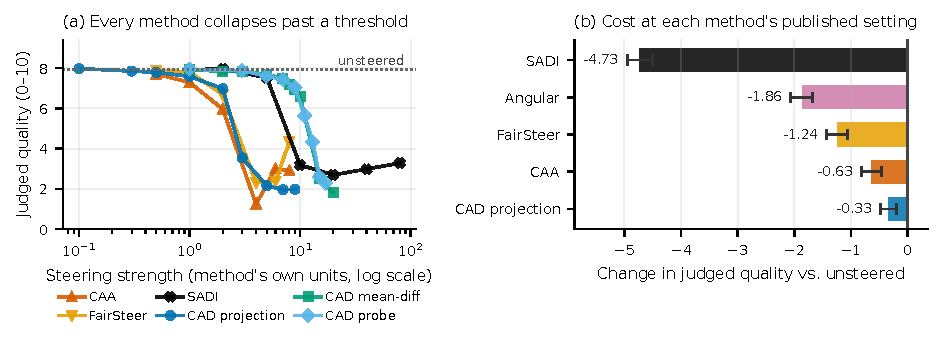
\includegraphics[width=\textwidth]{figure-02-collapse-and-cost.pdf}
\caption{(a) Judged quality against steering strength, one configuration family per
method so that only strength varies. Strengths are in each method's own units and
compare in shape rather than magnitude. Angular Steering is excluded because its
parameter is an angle and has no monotone ordering: $270^\circ$ is not a stronger dose
than $150^\circ$. (b) Quality change at each published setting, with bootstrap $95\%$
intervals.}
\label{fig:collapse}
\end{figure*}


\end{document}
